\section{Experiments}\label{sec:experiments}

\subsection{Setup}\label{sec:exp-setup}

All runs took place on November 16--17, 2026, with Claude Haiku~5.5 (Haiku) and Claude Sonnet~5.5 (Sonnet) as sub-agents; no Opus sub-agents were used. A configuration is one model at one effort level. Experiment~1 isolates unaided reasoning: the agent has no tools and cannot run code or check itself. Experiments~2 and~3 give the agent tools, tests and a working copy of a repository. Experiment~2 sweeps all ten configurations over twelve easy tasks, one trial per cell. Experiment~3 narrows to five configurations (Haiku \texttt{low}; Sonnet \texttt{low}, \texttt{medium}, \texttt{high}, \texttt{xhigh}) and ten harder tasks with three trials per cell, because the easy set barely separated configurations.

Experiment~1 comprised 229 runs and 1.71~million output tokens, in two stages. Experiment~2 comprised 120 runs. Experiment~3 comprised 150 runs and finished in 27~minutes on eight parallel slots. Dollar figures are API-equivalent (Section~\ref{sec:cost-accounting}).

\subsection{Reasoning without tools}\label{sec:exp-reasoning}

Each of three families (long multiplication, tracing generated Python, and a seating puzzle with a unique solution) has ten difficulty levels. We ran eight configurations (both models at \texttt{low}, \texttt{medium}, \texttt{high} and \texttt{xhigh}), one trial per cell, with tools forbidden and every transcript checked to contain only thinking and text. Levels 6--10 ran as chains that stopped after two consecutive failures, counting a failure at level 5, so ``longest solved at all'' means the longest level reached before a chain stopped; Haiku \texttt{low}'s trace levels above 250 statements were never run.

\paragraph{Results by family.} Seating logic gave no signal: every configuration solved every level, up to 13 people. In multiplication, every configuration solved up to $40 \times 40$ digits except Haiku \texttt{low}, which first failed at 25 digits, and Haiku \texttt{medium}, which first failed at 32. Both wrong answers had the right length and were correct except for one span of 8 to 10 digits, which held the right digits in the wrong order. Both configurations then solved the 40-digit problem, so these were not clean ceilings. Code tracing separated the configurations (Table~\ref{tab:trace} and Figure~\ref{fig:reasoning-trace}). Sonnet \texttt{xhigh} never failed. Sonnet \texttt{low} and \texttt{medium} reached 400 statements before failing. Haiku \texttt{high} and \texttt{xhigh} failed at 40 statements, earlier than Haiku \texttt{low} or \texttt{medium}, so effort did not help Haiku monotonically.

\begin{table}[H]
\centering
\caption{Code trace: longest program (in statements) solved before the first failure and at all, per configuration. ``1,300+'' means the top level was solved with no failure.}
\label{tab:trace}
\small
\begin{tabular}{l r r l}
\toprule
\textbf{Config} & \textbf{Before first failure} & \textbf{At all} & \textbf{Notes} \\
\midrule
Haiku \texttt{low}     & 80      & 80    & Failed 160 and 250 \\
Haiku \texttt{medium}  & 250     & 250   & Failed 400 and 600 \\
Haiku \texttt{high}    & 20      & 250   & Failed 40, 400, 600 \\
Haiku \texttt{xhigh}   & 20      & 400   & Failed 40 and 600; declined 900 \\
Sonnet \texttt{low}    & 400     & 400   & Failed 600 and 900 \\
Sonnet \texttt{medium} & 400     & 400   & Failed 600 and 900 \\
Sonnet \texttt{high}   & 400     & 900   & Failed 600, solved 900, failed 1,300 \\
Sonnet \texttt{xhigh}  & 1,300+  & 1,300 & Never failed \\
\bottomrule
\end{tabular}
\end{table}

\begin{figure}[H]
\centering
% Generated by analysis/make_tikz_figures.py. Edit the script, not this file.
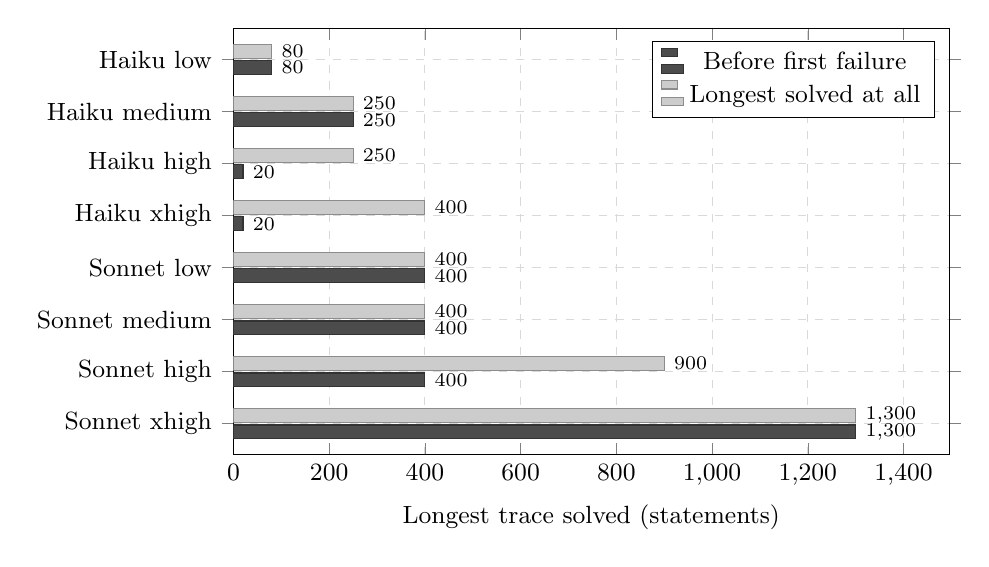
\begin{tikzpicture}
\begin{axis}[
  width=0.88\linewidth,
  height=7cm,
  grid=major,
  grid style={dashed, gray!30},
  tick label style={font=\small},
  label style={font=\small},
  xbar,
  bar width=5pt,
  xmin=0,
  xmax=1495,
  xtick distance=200,
  xlabel={Longest trace solved (statements)},
  ytick={8,7,6,5,4,3,2,1},
  yticklabels={Haiku low,Haiku medium,Haiku high,Haiku xhigh,Sonnet low,Sonnet medium,Sonnet high,Sonnet xhigh},
  ymin=0.4,
  ymax=8.6,
  nodes near coords,
  every node near coord/.append style={font=\scriptsize},
  legend style={at={(0.98,0.97)}, anchor=north east, font=\small},
]
\addplot[fill=black!70, draw=black!80, bar shift=-3pt] coordinates {(80,8) (250,7) (20,6) (20,5) (400,4) (400,3) (400,2) (1300,1)};
\addlegendentry{Before first failure}
\addplot[fill=black!20, draw=black!45, bar shift=3pt] coordinates {(80,8) (250,7) (250,6) (400,5) (400,4) (400,3) (900,2) (1300,1)};
\addlegendentry{Longest solved at all}
\end{axis}
\end{tikzpicture}

\caption{Longest code trace solved before the first failure and at all, per configuration. Values are statement counts.}
\label{fig:reasoning-trace}
\end{figure}

\paragraph{The swap shortcut.} At 40 statements, Haiku \texttt{high} and \texttt{xhigh} gave the same wrong answer. The program contains three swaps of one pair of variables followed by one swap of a different pair; both configurations treated this as ``four swaps that cancel out.'' Haiku \texttt{low} and \texttt{medium} traced each line and were correct. The shared wrong answer is consistent with a shared habit of the model, but one pair of configurations at one level cannot rule out chance. With one trial per cell we also cannot say whether longer thinking causes the shortcut.

\paragraph{An unexplained answer.} At 600 statements, Sonnet \texttt{low} and \texttt{medium} gave the same wrong answer. To check, we replayed the program with each single statement skipped, its branch flipped, or its swap applied in sequence, using a script in the repository; none reproduces it, and the cause is unknown. By contrast, Haiku \texttt{high}'s wrong answer at 600 is reproduced exactly by skipping one statement.

\paragraph{A declined answer.} At 900 statements, Haiku \texttt{xhigh} noticed it had re-traced a block it had already done and declined to answer. Every other failure was a definite wrong answer. An orchestrator can catch a refusal more easily than a confident error, but it still used 216k output tokens and 680\,s.

\paragraph{What effort cost.} On the 400-statement trace, Sonnet \texttt{low}, \texttt{medium} and \texttt{high} used 8--9k output tokens in 43--46\,s. Sonnet \texttt{xhigh} used 28k in 131\,s, and Haiku \texttt{xhigh} used 70k in 214\,s. The 1,300-statement run by Sonnet \texttt{xhigh} used 95k output tokens and 439\,s.

\subsection{Coding: easy set}\label{sec:exp-easy}

The easy set has twelve tasks (three locate, two fix, four feature, three review), run at all ten configurations: 120 runs, with Sonnet \texttt{high} and Haiku \texttt{medium} run first as a pilot. After one harness-caused rerun (Haiku \texttt{high}, locate-2), every configuration passed every locate, fix and feature task. The original row is kept, marked superseded.

\paragraph{The separating review.} Only the two-bug review separated configurations. Every Haiku level, \texttt{low} through \texttt{max}, and Sonnet \texttt{xhigh} missed the planted shutdown-loop bug, each reporting a real, pre-existing flaw nearby instead. Sonnet \texttt{low}, \texttt{medium}, \texttt{high} and \texttt{max} found both bugs. Totals were therefore 12/12 for those four Sonnet configurations and 11/12 for Sonnet \texttt{xhigh} and every Haiku level.

\paragraph{The review-grading change.} Many pilot ``false alarms'' were real defects already in the original commits (a rendering gap and a shutdown-status bug), so extra reports no longer fail a run and the review score measures recall on planted bugs, not precision (Section~\ref{sec:grading}).

\begin{table}[H]
\centering
\caption{Easy set: dollars per successful task, output tokens over the twelve tasks, and agent seconds per run.}
\label{tab:easy-cost}
\small
\begin{tabular}{l r r r}
\toprule
\textbf{Config} & \textbf{\$ per success} & \textbf{Output tokens} & \textbf{Agent s per run} \\
\midrule
Haiku \texttt{low}     & 0.017 & 66k  & 34  \\
Haiku \texttt{medium}  & 0.025 & 95k  & 48  \\
Haiku \texttt{high}    & 0.040 & 154k & 68  \\
Haiku \texttt{xhigh}   & 0.092 & 324k & 130 \\
Haiku \texttt{max}     & 0.339 & 910k & 332 \\
Sonnet \texttt{low}    & 0.118 & 27k  & 35  \\
Sonnet \texttt{medium} & 0.116 & 30k  & 24  \\
Sonnet \texttt{high}   & 0.164 & 45k  & 34  \\
Sonnet \texttt{xhigh}  & 0.258 & 91k  & 64  \\
Sonnet \texttt{max}    & 0.895 & 549k & 327 \\
\bottomrule
\end{tabular}
\end{table}

\begin{figure}[H]
\centering
% Generated by analysis/make_tikz_figures.py. Edit the script, not this file.
\begin{tikzpicture}
\begin{axis}[
  width=0.88\linewidth,
  height=7cm,
  grid=major,
  grid style={dashed, gray!30},
  tick label style={font=\small},
  label style={font=\small},
  xbar,
  xmode=log,
  log origin=infty,
  xmin=0.01,
  xmax=1,
  xlabel={Cost per success (\$, log scale)},
  xtick={0.01,0.1,1},
  xticklabels={\$0.01,\$0.1,\$1},
  ytick={10,9,8,7,6,5,4,3,2,1},
  yticklabels={Haiku low,Haiku medium,Haiku high,Haiku xhigh,Haiku max,Sonnet low,Sonnet medium,Sonnet high,Sonnet xhigh,Sonnet max},
  ymin=0.4,
  ymax=10.6,
  bar width=7pt,
  point meta=rawx,
  nodes near coords={\$\pgfmathprintnumber[fixed,precision=3]{\pgfplotspointmeta}},
  every node near coord/.append style={font=\scriptsize},
]
\addplot[fill=arxivgray!60, draw=arxivgray, bar shift=0pt] coordinates {(0.0174,10) (0.0250,9) (0.0405,8) (0.0918,7) (0.3385,6)};
\addplot[fill=arxivblue, draw=arxivblue, bar shift=0pt] coordinates {(0.1184,5) (0.1156,4) (0.1638,3) (0.2584,2) (0.8954,1)};
\end{axis}
\end{tikzpicture}

\caption{Easy set: dollars per successful task by configuration.}
\label{fig:easy-cost}
\end{figure}

Table~\ref{tab:easy-cost} and Figure~\ref{fig:easy-cost} give cost. Haiku \texttt{low} was cheapest and passed as many tasks as every other Haiku level; \texttt{max} was the most expensive at both models and bought nothing here. No agent made a false ``tests pass'' claim, but no fix or feature failed, so that check was untested.

\subsection{Coding: hard set}\label{sec:exp-hard}

The hard set separates symptom, cause and test, or says little in the brief. The three fixes differ: one has a hidden, distant cause (the five tests that catch it are hidden, in four files); one has two bugs behind one symptom, with only one visible failing test; one has a bug report that blames the wrong component. Three features are large commit replays (up to 15 files, 602 lines and 32 hidden tests); two are easy-set features briefed in 70 and 115 words. Two reviews contain two and three deliberately planted faults that the existing tests do not catch. Each configuration ran 30 runs (10 tasks, 3 trials).

\begin{table}[H]
\centering
\caption{Hard set results per configuration (30 runs each). ``Set aside'' excludes the ambiguous review bug described in the text.}
\label{tab:hard-results}
\small
\setlength{\tabcolsep}{4pt}
\begin{tabular}{l r r r r r r}
\toprule
\textbf{Config} & \textbf{As graded} & \textbf{Set aside} & \textbf{Code changes} & \textbf{\$/success} & \textbf{Out. tokens} & \textbf{Agent s/run} \\
\midrule
Haiku \texttt{low}     & 29/30 & 30/30 & 24/24 & 0.041 & 427k & 78  \\
Sonnet \texttt{low}    & 26/30 & 29/30 & 23/24 & 0.207 & 168k & 36  \\
Sonnet \texttt{medium} & 27/30 & 29/30 & 24/24 & 0.210 & 194k & 43  \\
Sonnet \texttt{high}   & 27/30 & 30/30 & 24/24 & 0.259 & 244k & 58  \\
Sonnet \texttt{xhigh}  & 27/30 & 30/30 & 24/24 & 0.532 & 606k & 145 \\
\bottomrule
\end{tabular}
\end{table}

\begin{figure}[H]
\centering
% Generated by analysis/make_tikz_figures.py. Edit the script, not this file.
\begin{tikzpicture}
\begin{axis}[
  width=0.88\linewidth,
  height=7cm,
  grid=major,
  grid style={dashed, gray!30},
  tick label style={font=\small},
  label style={font=\small},
  xmin=0.4,
  xmax=5.6,
  xtick={1,2,3,4,5},
  xticklabels={Haiku low,Sonnet low,Sonnet medium,Sonnet high,Sonnet xhigh},
  x tick label style={font=\scriptsize},
  ymin=0.5,
  ymax=1.0,
  ytick={0.5,0.6,0.7,0.8,0.9,1.0},
  ylabel={Pass rate (passes/runs)},
  legend pos=south west,
]
\addplot[only marks, mark=*, color=arxivgray, error bars/.cd, y dir=both, y explicit] table[col sep=comma, x=x, y=y, y error plus=eplus, y error minus=eminus] {
x,y,eplus,eminus
1,0.9667,0.0273,0.1337
};
\addlegendentry{Haiku}
\addplot[only marks, mark=*, color=arxivblue, error bars/.cd, y dir=both, y explicit] table[col sep=comma, x=x, y=y, y error plus=eplus, y error minus=eminus] {
x,y,eplus,eminus
2,0.8667,0.0803,0.1637
3,0.9000,0.0650,0.1560
4,0.9000,0.0650,0.1560
5,0.9000,0.0650,0.1560
};
\addlegendentry{Sonnet}
\end{axis}
\end{tikzpicture}

\caption{Hard set pass rates as graded, with Wilson 95\,\% intervals.}
\label{fig:hard-pass}
\end{figure}

Table~\ref{tab:hard-results} and Figure~\ref{fig:hard-pass} summarize results. Every configuration solved all three fixes, both terse features and the 4- and 9-file features in all three trials. The Wilson intervals~\cite{wilson1927probable} overlap (29/30 is 83--99\,\%, 26/30 is 70--95\,\%), so as-graded gaps are weak evidence.

\paragraph{The 602-line feature.} Sonnet \texttt{low} failed it once, with seven failing tests. No other configuration failed a code change in any trial.

\paragraph{The ambiguous handler.} In the three-bug review, no Sonnet run at any effort level flagged the third planted bug: an error handler broadened to catch every exception, which turns parsing errors and code bugs into a quiet error instead of a crash. This is arguably a robustness choice rather than a defect, and the prompt asked only for real runtime defects. The answer key was written by a Sonnet sub-agent, not a person. We therefore count the runs both ways: as graded, and with this bug set aside. Eleven Sonnet runs found the other two bugs; one Sonnet \texttt{medium} run found only one, which counts against it under both views. Haiku \texttt{low} flagged the third bug in two of three runs. Three trials cannot show that Haiku is better at it.

\paragraph{False success claims and denials.} No false success claim was confirmed. The one flagged run was a harness anomaly (below), and the one real failure on a fix or feature did not claim success. The hard set recorded 189 denied tool calls: 154 chained commands (\texttt{;}, \texttt{||}, pipes, loops) that an allowlist cannot match, 15 other \texttt{uv} subcommands, 15 \texttt{sed -i}, and 5 others. (An earlier count of 234 double-counted results that transcripts repeat.) Agents retried with simpler commands or the edit tool, and no failure traced to a denial.

\paragraph{Harness problems.} We found and fixed three. First, in one Sonnet \texttt{high} run of the 602-line feature, a hidden test file was never collected during grading, so the run was graded a failure and flagged as a false claim. The grader now treats a hidden test file with no results as a harness error and retries. A fresh sample passed; the original row is kept, marked superseded. Second, saved diffs omitted new files, so that run could not be replayed; they now include them. Third, the claim parser read an earlier baseline count instead of the final run's; it now uses the largest pytest-style count in the reply.

\subsection{Cost}\label{sec:exp-cost}

Dollars per success rose with effort above \texttt{medium} on both sets (Tables~\ref{tab:easy-cost} and~\ref{tab:hard-results}); Sonnet \texttt{medium} was slightly cheaper than Sonnet \texttt{low} on the easy set. Haiku \texttt{low} cost \$0.017 on the easy set and \$0.041 on the hard set; Sonnet \texttt{low} cost \$0.118 and \$0.207.

\paragraph{Haiku's price against its tokens and time.} Haiku costs about 1/20 as much per token as Sonnet but writes more and runs longer. Against Sonnet \texttt{low} on the hard set it used about 2.5 times the output tokens and about twice the agent time, and still cost about one fifth as much per success. The price is wall-clock: Sonnet \texttt{medium} took 43\,s per hard-set run and 24\,s per easy-set run, against 78\,s and 34\,s for Haiku \texttt{low}.

\paragraph{Effort above medium.} Sonnet \texttt{xhigh} cost about 2.2 times Sonnet \texttt{low} per success on the easy set and 2.6 times on the hard set. On the easy set, \texttt{max} cost about 8 times \texttt{low} for Sonnet and about 19 times for Haiku. Pass counts did not improve: Sonnet \texttt{xhigh} scored 11/12 on the easy set, one below Sonnet \texttt{low}. Figure~\ref{fig:effort-cost} plots the easy-set curve, and Figure~\ref{fig:hard-cost-time} plots dollars against agent time on the hard set. Because nearly every task passed at every configuration, the absence of an effort benefit may be a ceiling effect. The coding runs cost about \$24 (easy set) and \$34 (hard set).

\begin{figure}[H]
\centering
% Generated by analysis/make_tikz_figures.py. Edit the script, not this file.
\begin{tikzpicture}
\begin{axis}[
  width=0.88\linewidth,
  height=7cm,
  grid=major,
  grid style={dashed, gray!30},
  tick label style={font=\small},
  label style={font=\small},
  xtick={1,2,3,4,5},
  xticklabels={low,medium,high,xhigh,max},
  xmin=0.6,
  xmax=5.4,
  xlabel={Effort level},
  ymode=log,
  ymin=0.01,
  ymax=1,
  ytick={0.01,0.1,1},
  yticklabels={\$0.01,\$0.1,\$1},
  ylabel={Cost per success (\$, log scale)},
  legend pos=south east,
  typeset ticklabels with strut,
]
\addplot[color=arxivgray, mark=*, thick] coordinates {(1,0.0174) (2,0.0250) (3,0.0405) (4,0.0918) (5,0.3385)};
\addlegendentry{Haiku}
\addplot[color=arxivblue, mark=square*, thick] coordinates {(1,0.1184) (2,0.1156) (3,0.1638) (4,0.2584) (5,0.8954)};
\addlegendentry{Sonnet}
\end{axis}
\end{tikzpicture}

\caption{Easy set: dollars per success against effort level, one line per model.}
\label{fig:effort-cost}
\end{figure}

\begin{figure}[H]
\centering
% Generated by analysis/make_tikz_figures.py. Edit the script, not this file.
\begin{tikzpicture}
\begin{axis}[
  width=0.88\linewidth,
  height=7cm,
  grid=major,
  grid style={dashed, gray!30},
  tick label style={font=\small},
  label style={font=\small},
  xmin=0,
  xmax=180.8,
  ymin=0,
  ymax=0.665,
  xlabel={Agent seconds per run},
  ylabel={Cost per success (\$)},
  legend pos=north west,
]
\addplot[only marks, mark=*, color=arxivgray, nodes near coords, point meta=explicit symbolic, visualization depends on={value \thisrow{anchor} \as \labelanchor}, every node near coord/.append style={anchor=\labelanchor, font=\scriptsize}] table[col sep=comma, x=x, y=y, meta=label] {
x,y,label,anchor
77.6,0.0410,Haiku low,west
};
\addlegendentry{Haiku}
\addplot[only marks, mark=*, color=arxivblue, nodes near coords, point meta=explicit symbolic, visualization depends on={value \thisrow{anchor} \as \labelanchor}, every node near coord/.append style={anchor=\labelanchor, font=\scriptsize}] table[col sep=comma, x=x, y=y, meta=label] {
x,y,label,anchor
36.0,0.2071,Sonnet low,east
43.2,0.2097,Sonnet medium,south
58.0,0.2593,Sonnet high,west
144.6,0.5323,Sonnet xhigh,east
};
\addlegendentry{Sonnet}
\end{axis}
\end{tikzpicture}

\caption{Hard set: dollars per success against agent seconds per run.}
\label{fig:hard-cost-time}
\end{figure}
